\begin{remark}
    Section made from lectures done by Jøran Moen. Other sources are \citet{1995Itsp} --- chapter 11.
\end{remark}
\noindent\textbf{This week:}
\begin{enumerate}[\(\bullet \)]
    \item guess harmonic oscillations
    \item derive dispersion relation
    \item identify wave modes\begin{enumerate}[\(\triangleright \)]
        \item plasma acoustic
        \item Alfvén
        \item magnetosonic
    \end{enumerate}
    \item energy sources
\end{enumerate}
\section{MHD-equations: introduction}
The MHD-waves are ULF waves, i.e.~\(f<f_p,f_{ci}\), where
\begin{equation*}
    f_p=\frac{1}{2\pi}\sqrt{\frac{ne^2}{\epsilon_0m}},\quad f_{ci}=\frac{1}{2\pi}\frac{qB}{m}
\end{equation*}
is the plasma and ion gyro frequencies respectively. We remind ourself of the MHD equations, \cref{eq:MHD_1,eq:MHD_2,eq:MHD_3,eq:MHD_4,eq:MHD_5,eq:MHD_6}. From these six, we may combine them to reduce the number of equations to five. We then end up with
\begin{align}
    \p{t}{\rho}+\nabla\cdot\left(\rho \gf{v}\right)&=0\label{eq:simple_MHD1}\\
    \rho\left[\p{t}{\gf{v}}+(\gf{v}\cdot\nabla)\gf{v}\right]&=-\nabla p-\frac{1}{\mu_0}\gf{B}\times\left(\nabla\times\gf{B}\right)\label{eq:simple_MHD2}\\
    \p{t}{\gf{B}}&=\nabla\times\left(\gf{v}\times\gf{B}\right)\label{eq:simple_MHD3}\\
    \nabla\cdot\gf{B}&=0\label{eq:simple_MHD4}\\
    p&=S\rho^\gamma\label{eq:simple_MHD5}
\end{align}
where \(S\) is the entropy and we have assumed frozen in conditions where \(\gf{E}\) can be written into \(\gf{v}\times\gf{B}\). We then linearize these equations by writing all parameters on the form \(\xi=\xi_0+\xi_1\) and only keeping terms of \(\orderof(1)\) or less. We want to rewrite the latter equation by finding the gradient, which gives
\begin{equation}\label{eq:simplify_MHD6}
    \begin{aligned}
        \nabla p_1&=S\gamma{\left(\rho_0+\rho_1\right)}^{\gamma-1}\nabla\rho_1\\
        &=\gamma\frac{p_0+p_1}{\rho_0+\rho_1}\nabla\rho_1,\quad p_0\gg p_1, \rho_0\gg\rho_1\\
        &=\gamma\frac{p_0}{\rho_0}\nabla\rho_1=c_s^2\nabla\rho_1
    \end{aligned}
\end{equation}
where we have used that \(S=\left(p_0+p_1\right)/{\left(\rho_0+\rho_1\right)}^\gamma \). We assume normal mode solutions, i.e.\ we write \(\xi_1=\widetilde{\xi}e^{i\left(\gf{k}\cdot\gf{r}-\omega t\right)}\), where \(\xi_1\) may be either a scalar or a vector.

\section{Acoustic wave}
We can reduce our five equations even further by choosing to neglect both the electric and the magnetic field, leaving only the top two equations. We use the result from \cref{eq:simplify_MHD6} and plug it into \cref{eq:simple_MHD2}, and then replace all parameters with normal mode solutions. Doing all this yields
\begin{align*}
    -i\omega\rho_1+\rho_0i\gf{k}\cdot\gf{u}_1=0\\
    i\omega\rho_0\gf{u}_1=-i\gf{k}c_s^2\rho_1
\end{align*}
From here, we can find the dispersion relation we were looking for, given as
\begin{equation*}
    \omega^2=k_x^2C_s^2
\end{equation*}
where we have defined \(\gf{k}=k_x\f{x}\) and \(C_s\) is the phase velocity.

\section{Waves in cold plasma}
We now write the pressure as
\begin{align*}
    p&=n_{i}k_{B}T_i+n_{e}k_{B}T_e\\
    p_B&=\frac{B^2}{2\mu_0}
\end{align*}
where \(p_B\) is the magnetic pressure. If the magnetic field dominate the pressure, we express this with the parameter
\begin{equation*}
    \beta=\frac{p}{p_B}=\frac{p}{B^2/2\mu_0}\ll 1
\end{equation*}
The MHD equations for a cold plasma is as given in \cref{eq:simple_MHD1,eq:simple_MHD2,eq:simple_MHD3,eq:simple_MHD4,eq:simple_MHD5}, but where \(\nabla p\rightarrow 0\), i.e.\ \cref{eq:simple_MHD1,eq:simple_MHD2,eq:simple_MHD3} are the relevant equations.

\section{Exercises}
\begin{enumerate}
    \item [\textbf{EXERCISE 1 --- Exam 2004}]~\vspace{1pt}\begin{enumerate}[(a)]
        \item Assume a static uniform magnetic field oriented along the \(y\)-axis with a static electric field along the \(z\)-axis. Define your coordinate system and sketch the particle trajectories separately for electrons and ions. Clearly indicate the direction of movement.
        \mylinbrk{}
        The movement is illustrated in \cref{fig:L7_ExB}.
        \item Assume a magnetic field along the \(z\)-direction increasing in strength along positive \(y\)-direction. Sketch the particle trajectories for the ions and electrons.
        \mylinbrk{}
        The movement is illustrated in \cref{fig:L7_gradB}.
        \item Which of the two situations above give rise to currents in plasmas with equal numbers of positive and negative charges?
        \mylinbrk{}
        Only the situation in \subref{fig:L7_gradB} will give a current given equal amount of positive and negative charges.
        \item The radius of the magnetic field is defined as
        \begin{equation*}
            \frac{\gf{R}_c}{||\gf{R}_c||}
        \end{equation*}
        which is pointing from the centre of the Earth perpendicular to \(\gf{B}\). Draw a sketch of the geometry in the Earth meridian plane, and derive the expression for the curvature drift given as:
        \begin{equation*}
            \gf{u}_c=\frac{mv_{||}^2}{qB^2}\frac{\gf{R}_c\times\gf{B}}{R_c^2}
        \end{equation*}
        \mylinbrk{}
        Sketch of the geometry is in \cref{fig:L7_curvB}. The curvature drift can be derived by looking at the centrifugal force and plugging it into the general expression for the drift velocity, given by \cref{eq:gen_v_drift}. The centrifugal force is given as
        \begin{equation*}
            m\gf{a}_{||}=m\frac{v_{||}^2}{\gf{R}_c}
        \end{equation*}
        Plugging this into \cref{eq:gen_v_drift} gives
        \begin{equation*}
            \gf{u}_c=m\frac{v_{||}^2}{R_c^2}\frac{\gf{R}_c\times\gf{B}}{qB^2}
        \end{equation*}
        which is what we wanted to find.
        \item The gradient drift velocity is given as:
        \begin{equation*}
            \gf{u}_{\nabla B}=\frac{1}{2}mv_\perp^2\frac{\gf{B}\times\nabla B}{qB^3}
        \end{equation*}
        Suppose the Earth's magnetic field is \(\num{3e-5}\si{\tesla}\) at the equator and falls off as \(1/r^3\). Let there be an isotropic population of \SI{30}{\kilo\electronvolt} protons and \SI{30}{\kilo\electronvolt} electrons, each with a density of \(n=10^{-7}\si{\metre^{-3}}\) at \(r=5R_E\) in the equatorial plane. (\(m_i=\num{1.67e-27}\si{\kilo\gram}\), \(m_e=\num{9.11e-31}\si{\kilo\gram}\), \(q=\num{1.6e-19}\si{\coulomb}\) and \(R_c=r=5\)).

        Calculate the ion and electron \(\nabla B\) and curvature drifts. In what direction is the ring current encircling the Earth? Justify your answer.
        \mylinbrk{}
        Since the energy is said to be isotropic, we know that \(mv_{||}^2/2=\SI{30}{\kilo\electronvolt}\) and \(mv_\perp^2=\SI{60}{\kilo\electronvolt}\). We also need to find the gradient of the magnetic field in the radial direction. Since it decreases as \(1/r^3\) we get
        \begin{equation*}
            \p{r}{B}=-\frac{-3C}{r^4}
        \end{equation*}
        where \(C\) is a constant given as
        \begin{equation*}
            B(R_E)=\frac{C}{R_E^3}=\num{3e-5}\si{\tesla}\Rightarrow C=\num{7.86e15}\si{\tesla\metre^3}
        \end{equation*}
        The velocity due to \(\nabla B\) will be
        \begin{equation*}
            u_{\nabla B}=\frac{1}{2}mv_\perp^2\frac{1}{q}\frac{\nabla B}{B^2}=\frac{1}{2}mv_\perp^2\frac{3C}{r^4}\frac{r^6}{C^2}\approx\SI{11.7}{\kilo\metre/\second}
        \end{equation*}
        For the curvature drift, we get
        \begin{equation*}
            u_c=\frac{mv_{||}^2}{qB}\frac{B}{R_c}\approx\SI{7.8}{\kilo\metre/\second}
        \end{equation*}
        \item Compute the ring current density in \si{\ampere\metre^{-2}}. At what fraction does the \(\nabla B\) drift of ions contribute?
        \mylinbrk{}
        Here, we use the equation for the current given as
        \begin{equation*}
            j=ne\left(v_i-v_e\right)
        \end{equation*}
        but we also need to remember that we get double contribution since we have both ions and electrons. I.e.\ we get
        \begin{equation*}
            j=2ne\left(u_{\nabla B}+u_c\right)=\num{6.25e-22}\si{\ampere/\metre^2}
        \end{equation*}
        The contribution from the \(\nabla B\) drift of ions can be found to be
        \begin{equation*}
            \tn{Ion contribution}=\frac{\SI{11.7}{\kilo\metre/\second}}{2\times\SI{11.7}{\kilo\metre/\second}+2\times\SI{7.8}{\kilo\metre/\second}}=30\%
        \end{equation*}
    \end{enumerate}
    \begin{figure}[t]
        \centering

        \begin{subfigure}[t]{.3\linewidth}
            \centering
            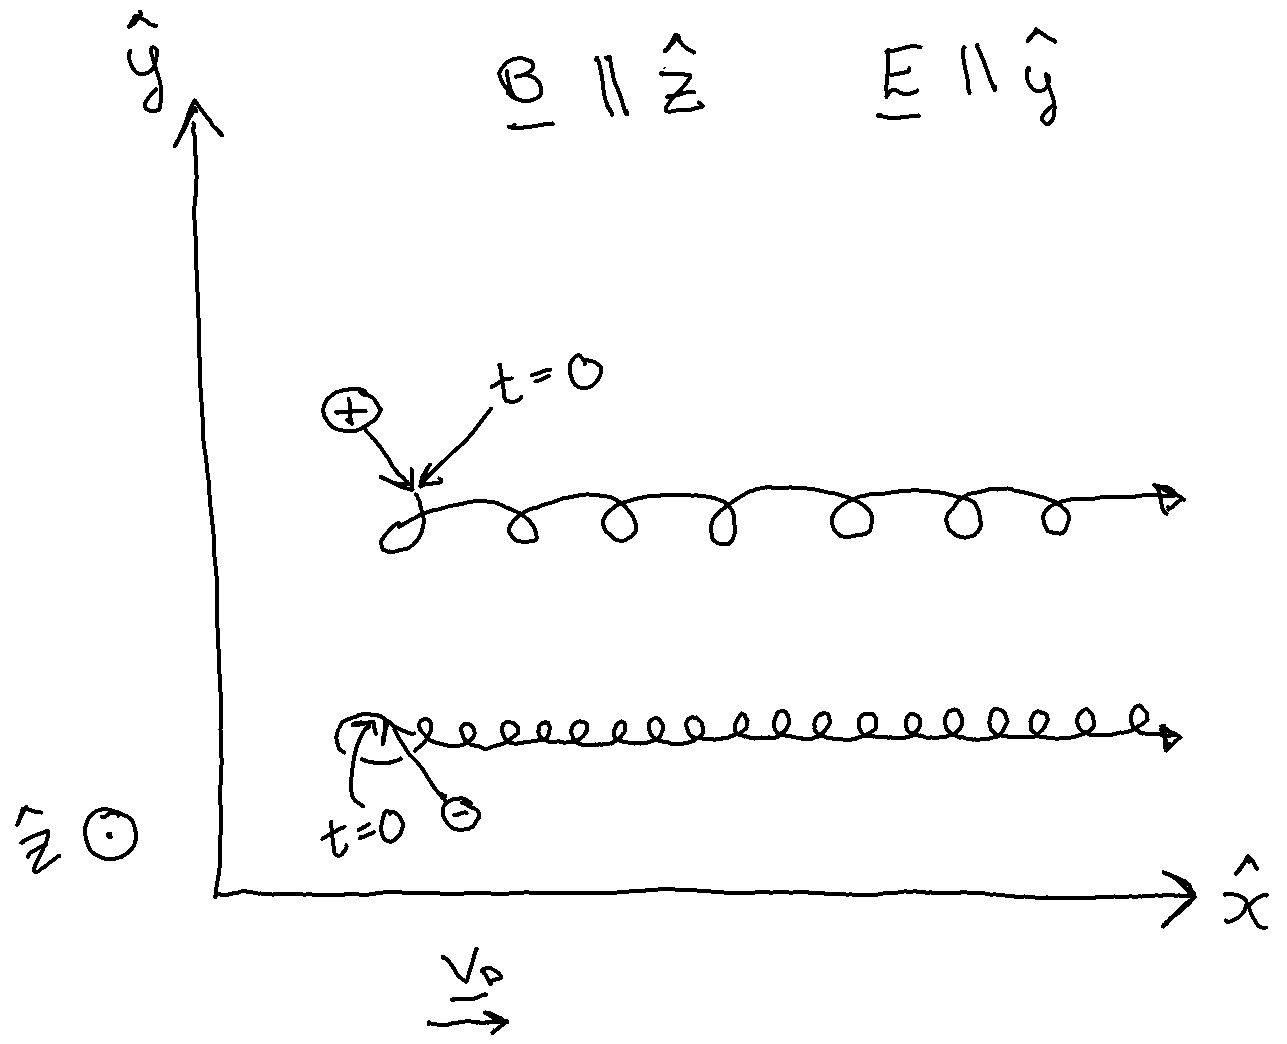
\includegraphics[width=.95\linewidth]{bilder/L7_ExB.png}
            \caption{}\label{fig:L7_ExB}
        \end{subfigure}
        \begin{subfigure}[t]{.3\linewidth}
            \centering
            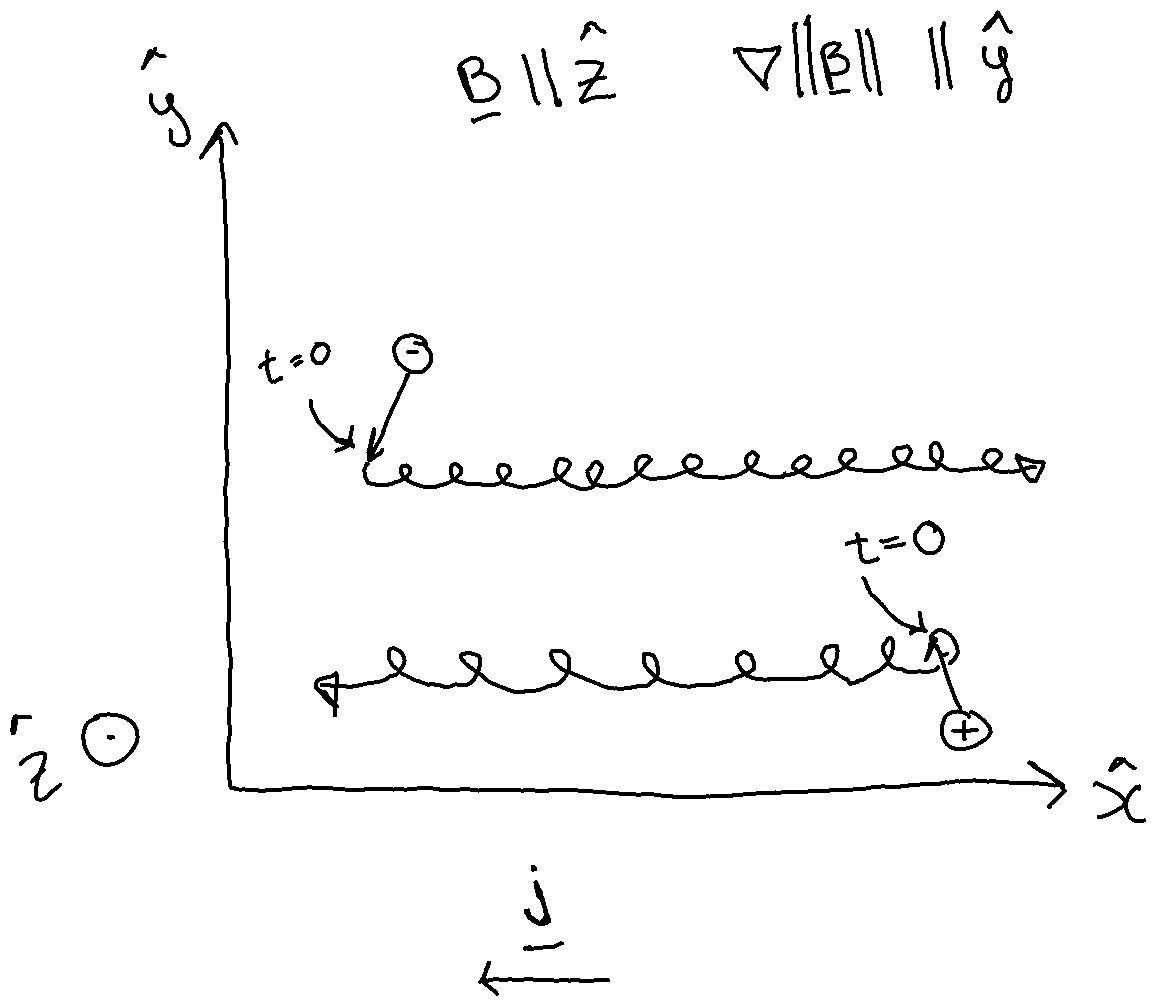
\includegraphics[width=.95\linewidth]{bilder/L7_gradB.png}
            \caption{}\label{fig:L7_gradB}
        \end{subfigure}
        \begin{subfigure}[t]{.3\linewidth}
            \centering
            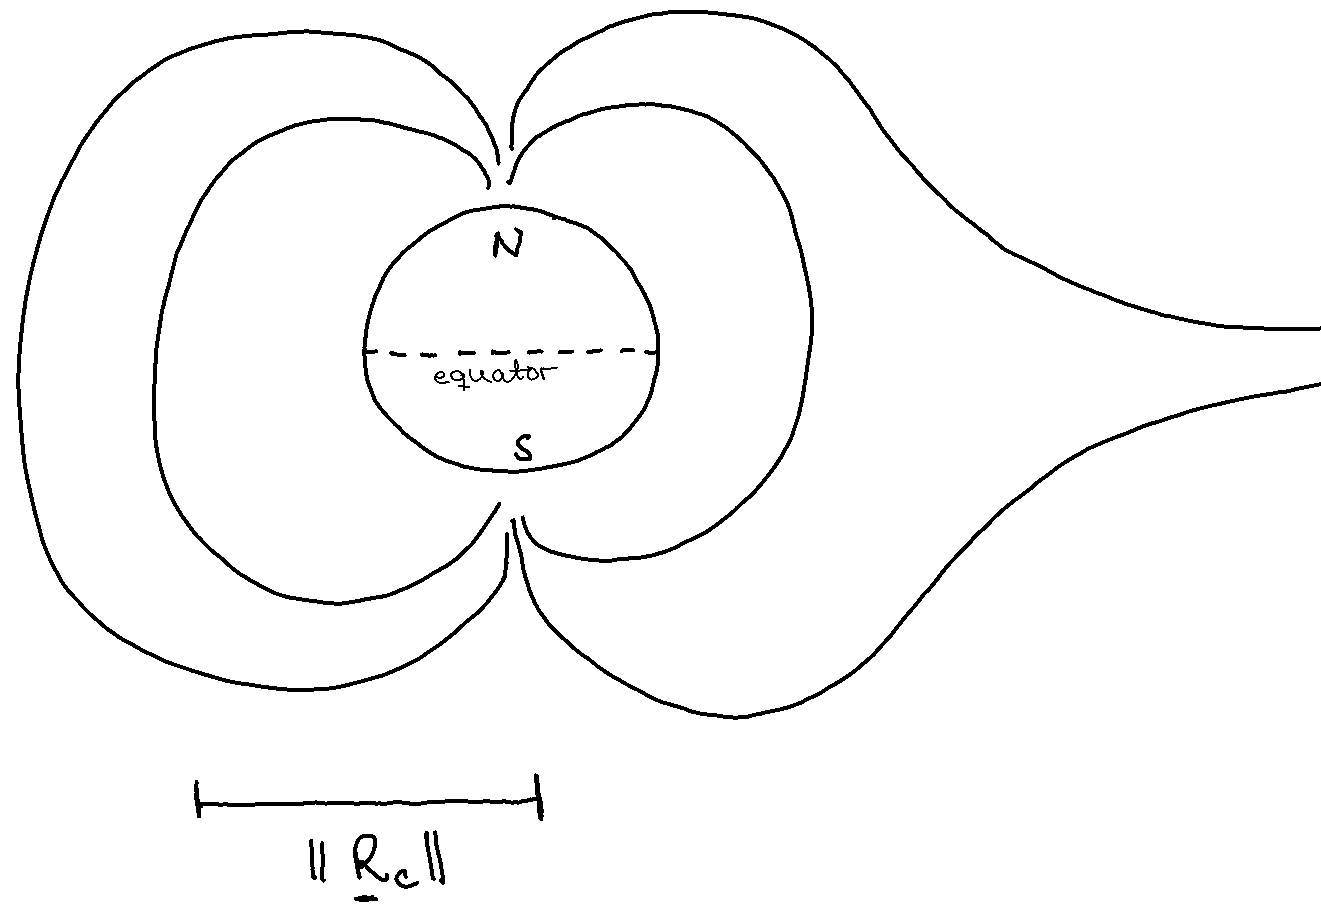
\includegraphics[width=.95\linewidth]{bilder/L7_curvB.png}
            \caption{}\label{fig:L7_curvB}
        \end{subfigure}

        \caption{Three nice drawings.}\label{fig:L7_ex1}
    \end{figure}
    \item [\textbf{EXERCISE 2 --- Prob. 5 Exam 1996}] The set of linearized equations for a cold plasma approximation is given by
    \begin{align*}
        \p{t}{\rho_1}+\nabla\cdot\left(\rho_0 \gf{v}_1\right)&=0\\
        \rho_0\p{t}{\gf{v}_1}&=-\frac{1}{\mu_0}\gf{B}_0\times\left(\nabla\times\gf{B}_1\right)\\
        \p{t}{\gf{B}_1}&=\nabla\times\left(\gf{v}_1\times\gf{B}_0\right)
    \end{align*}
    \begin{enumerate}[(a)]
        \item What is the essential assumption for the ``cold'' plasma approximation?
        \mylinbrk{}
        The essential assumption for a cold plasma approximation is that it is cold enough for pressure to be neglected. Pressure differences can't propagate.
        \item Let us introduce a small perturbation in the plasma, \(\gf{u}=\gf{u}_1\), \(\rho=\rho_0+\rho_1\), \(\gf{B}=\gf{B_0}+\gf{B_1}\). Linearize the set of MHD-equations under the assumption that the background magnetic field and the plasma density are constant.
        \mylinbrk{}
        The linearization is done already.
        \item We want to derive the dispersion relation for a cold plasma given the equations above. We assume normal mode solutions and rewrite the differential operators to get
        \begin{align*}
            -i\omega\rho_1+i\rho_0\gf{k}\cdot\gf{\widetilde{v}}_1&=0\\
            -i\omega\rho_0\gf{\widetilde{v}}_1&=-\frac{1}{\mu_0}\gf{\widetilde{B}}_0\times\left(i\gf{k}\times\gf{\widetilde{B}}_1\right)\\
            -i\omega\gf{\widetilde{B}}_1&=i\gf{k}\times\left(\gf{\widetilde{v}}_1\times\gf{\widetilde{B}}_0\right)
        \end{align*}
        By using the well known vector identity, the triple vector product \(\gf{A}\times\left(\gf{B}\times\gf{C}\right)=\left(\gf{A}\cdot\gf{C}\right)\gf{B}-\left(\gf{A}\cdot\gf{B}\right)\gf{C}\), and by letting \(\gf{k}=k\f{x}\) we can write this as
        \begin{align}
            -\omega\rho_1+\rho_0kv_{1x}&=0\label{eq:L7_alfven_normalmode1}\\
            -\omega\rho_0\gf{\widetilde{v}}_1&=-\frac{1}{\mu_0}\left[\left(\gf{\widetilde{B}}_0\cdot\gf{\widetilde{B}}_1\right)k\f{x}-B_{0x}k\gf{\widetilde{B}}_1\right]\label{eq:L7_alfven_normalmode2}\\
            -\omega\gf{\widetilde{B}}_1&=kB_{0x}\gf{v}_1-kv_{1x}\gf{\widetilde{B}}_0\label{eq:L7_alfven_normalmode3}
        \end{align}
        We choose our coordinate system such that \(\gf{\widetilde{B}}_0=\left[B_0\cos\theta,0,B_0\sin\theta\right]\), which yields
        \begin{align*}
            -\omega\rho_1+\rho_0kv_{1x}&=0\\
            -\omega\rho_0\gf{\widetilde{v}}_1&=-\frac{1}{\mu_0}\left[\left(B_{1x}B_0\cos\theta+B_{1z}B_0\sin\theta\right)k\f{x}-B_{0}\cos\theta k\gf{\widetilde{B}}_1\right]\\
            \gf{\widetilde{B}}_1&=\frac{-1}{\omega}kB_{0}\cos\theta\gf{v}_1+\frac{1}{\omega}kv_{1x}\gf{\widetilde{B}}_0
        \end{align*}
        where we can decompose \(\gf{\widetilde{B}}_1\) into
        \begin{equation*}
            \left(\begin{array}{c}
                B_{1x}\\
                B_{1y}\\
                B_{1z}
            \end{array}\right)=\frac{1}{\omega}\left(\begin{array}{c}
                B_0kv_{1x}\cos\theta-B_0kv_{1x}\cos\theta \\
                0-B_0kv_{1y}\cos\theta \\
                B_0kv_{1x}\sin\theta-B_0kv_{1z}\cos\theta
            \end{array}
            \right)
        \end{equation*}
        where we notice that \(B_{1x}=0\). Plugging this into our second equation yields
        \begin{equation*}
            \frac{\omega^2}{k^2}\gf{\widetilde{v}}_1=\frac{1}{\rho_0\mu_0}\left[\left(B_0v_{1x}\sin\theta-B_0v_{1z}\cos\theta\right)B_0\sin\theta\f{x}-B_{0}\cos\theta\left(
                \begin{array}{c}
                    0\\
                    -B_0v_{1y}\cos\theta \\
                    B_0v_{1x}\sin\theta-B_0v_{1z}\cos\theta
                \end{array}
                \right)\right]
        \end{equation*}
        The left hand side have all components of \(\gf{\widetilde{v}}_1\) in one term, while the right hand side have terms that include one of the components only in a given term. We move everything over to the left hand side and write the equation on matrix form with respect to the velocity vector. By doing this we obtain
        \begin{equation}\label{eq:L7_alfven_matrix_form}
            \left(
                \begin{array}{ccc}
                    \frac{\omega^2}{k^2}-\frac{B_0^2}{\rho_0\mu_0}\sin^2\theta &0&\frac{B_0^2}{\rho_0\mu_0}\cos\theta\sin\theta \\
                    0&\frac{\omega^2}{k^2}-\frac{B_0^2}{\rho_0\mu_0}\cos^2\theta &0\\
                    \frac{B_0^2}{\rho_0\mu_0}\cos\theta\sin\theta &0&\frac{\omega^2}{k^2}-\frac{B_0^2}{\rho_0\mu_0}\cos^2\theta
                \end{array}
            \right)\left(\begin{array}{c}
                    v_{1x}\\
                    v_{1y}\\
                    v_{1z}
                \end{array}
            \right)=\gf{0}
        \end{equation}
        where
        \begin{equation*}
            v_A^2=\frac{B_0^2}{\rho_0\mu_0},\quad\tn{Alfvén speed}
        \end{equation*}
        The dispersion relation can now very simply be found by assuming no trivial solutions exist. This means that the determinant of the matrix must be zero, hence
        \begin{equation*}
        \begin{aligned}
            \det\left(
                \begin{array}{ccc}
                    \frac{\omega^2}{k^2}-\frac{B_0^2}{\rho_0\mu_0}\sin^2\theta &0&\frac{B_0^2}{\rho_0\mu_0}\cos\theta\sin\theta \\
                    0&\frac{\omega^2}{k^2}-\frac{B_0^2}{\rho_0\mu_0}\cos^2\theta &0\\
                    \frac{B_0^2}{\rho_0\mu_0}\cos\theta\sin\theta &0&\frac{\omega^2}{k^2}-\frac{B_0^2}{\rho_0\mu_0}\cos^2\theta
                \end{array}
            \right)=0\\
            \left(\frac{\omega^2}{k^2}-v_A^2\cos^2\theta\right)\left(\frac{\omega^2}{k^2}-v_A^2\right)=0
        \end{aligned}
        \end{equation*}
        We see that this has two solutions, which will manifest themselves as two different Alfvén modes, namely
        \begin{align}
            \frac{\omega^2}{k^2}=v_A^2\cos^2\theta\quad&\sim\quad\tn{shear Alfvén wave mode}\label{eq:L7_shear_alfven_mode}\\
            \frac{\omega^2}{k^2}=v_A^2\quad&\sim\quad\tn{compressional wave mode}\label{eq:L7_compression_mode}
        \end{align}
        In the figure from \citet{1995Itsp}, they use a Poynting flux vector, defined as \(\gf{S}=\frac{1}{\mu_0}\gf{E}_1\times\gf{B}_1\), showing the direction of the propagation of the wave energy. We can investigate this further, plugging \cref{eq:L7_shear_alfven_mode} into the top row of \cref{eq:L7_alfven_matrix_form}. This gives
        \begin{equation*}
            \left(v_A^2\cos^2\theta-v_A^2\sin^2\theta\right) v_{1x}+v_A^2\cos\theta\sin\theta v_{1z}=0
        \end{equation*}
        Doing the same with the bottom row will lead to the implication that \(v_{1x}=v_{1z}=0\) while \(v_{1y}\) can take any value. But from \cref{eq:L7_alfven_normalmode1} we see that \(v_{1x}=0 \Rightarrow \rho_1=0\). It also affect \cref{eq:L7_alfven_normalmode3}, in which \(v_{1x}=0 \Rightarrow \gf{B}_1\vert\vert\gf{v}_1\perp\gf{B}_0\). We can then look at the size of the components \(\gf{B}_0\) and \(\gf{B}_1\)
        \begin{equation*}
            \left\vert\gf{B}_0+\gf{B}_1\right\vert=B_0^2+\underbrace{2\gf{B}_0\cdot\gf{B}_1}_{=0}+\cancelto{0}{B_1^2}
        \end{equation*}
        \(\therefore \) Magnetic pressure is constant.
        \item In the case of warm plasma the dispersion relation is given by:
        \begin{equation*}
            \left(\omega^2-k^2v_A^2\cos^2\theta\right)\left[\omega^4-\omega^2k^2\left(c_s^2+v_A^2\right)+k^4v_A^2c_s^2\cos^2\theta\right]=0
        \end{equation*}
        Identify the possible solutions/wave modes and discuss the Friedrich's diagram for the phase velocity, as shown in the top left diagram in \cref{fig:L7_alfven_waves}, i.e.\ the case where \(v_A=2c_s\).
        \mylinbrk{}
        What we see is that the two modes are recognized as
        \begin{align*}
            \frac{\omega^2}{k^2}&=v_A^2\cos^2\theta \\
            \frac{\omega^2}{k^2}&=\frac{1}{2}\left \{c_s^2+v_A^2\pm \sqrt{{\left(c_s^2+v_A^2\right)}^2-4c_s^2v_A^2\cos^2\theta}\right \}
        \end{align*}
        where the first dispersion relation give the intermediate mode and the second give the fast and slow modes. Looking closer at the second dispersion relation, we notice that if
        \begin{align*}
            \theta=0:\quad\frac{\omega^2}{k^2}&=\frac{1}{2}\left \{c_s^2+v_A^2\pm\left(c_s^2-v_A^2\right)\right \} \\
            \theta=\frac{\pi}{2}:\quad\frac{\omega^2}{k^2}&=\frac{1}{2}\left \{c_s^2+v_A^2\pm\left(c_s^2+v_A^2\right)\right \}
        \end{align*}
        \begin{minipage}{.4\linewidth}
            \begin{align*}
                \theta&=0 \rightarrow \gf{k}||\gf{B}\\
                \frac{\omega^2}{k^2}&=v_A^2\\
                \frac{\omega^2}{k^2}&=c_s^2
            \end{align*}
        \end{minipage}
        \begin{minipage}{.4\linewidth}
            \begin{align*}
                \theta&=\frac{\pi}{2} \rightarrow \gf{k}\perp\gf{B}\\
                \frac{\omega^2}{k^2}&=c_s^2+v_A^2~\tn{(FAST)}\\
                \frac{\omega^2}{k^2}&=0~\tn{(SLOW)}
            \end{align*}
        \end{minipage}
        \item Waves generated at the magnetopause can be observed behind Earth's bow shock. Only one of the MHD wave modes modes can travel from the magnetopause to the nose of the bow shock. Which wave mode is it? Qualify our answer.
        \mylinbrk{}
        My guess is that, since moving from the magnetopause to the bow shock means moving through the IMF, which then means the wave moves with a component perpendicular to the IMF, only the fast mode will be able to propagate over.
    \end{enumerate}
\end{enumerate}
\begin{figure}[t]
    \centering
    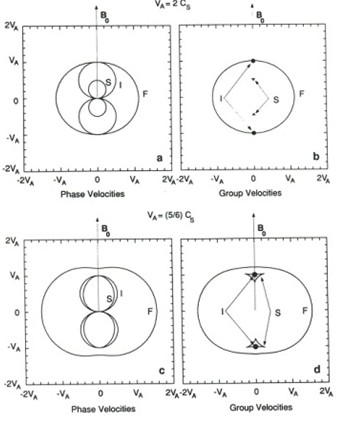
\includegraphics[width=.6\linewidth]{bilder/L7_alfven_waves.jpg}
    \caption{The fast (F), slow (S) and Alfvén wave (I) for \(v_A=2v_S\) (top) and \(v_A=5/6v_S\) (bottom).}\label{fig:L7_alfven_waves}
\end{figure}

\section[Standing waves]{Standing waves (K\&R 11.6)}
Let \(\ell=\) distance between the two ionospheres/hemispheres. A standing wave will then have
\begin{equation*}
    \lambda_{||}=\frac{2\ell}{n}
\end{equation*}
where \(n\in\mathbb{N}\) which is for a shear Alfvén wave. We also have
\begin{equation*}
    \frac{\omega}{k}=v_A\cos\theta\Rightarrow\frac{\omega}{k\cos\theta}=v_A=\frac{\omega}{k_{||}}
\end{equation*}
Further, we write \(k\) in terms of \(\lambda \) to gain information about the frequency.
\begin{equation*}
    f=\frac{\omega}{2\pi}=\frac{n\pi}{2\ell}v_A=\frac{n}{2\ell}\frac{B}{\sqrt{\mu_0\rho}}
\end{equation*}